% Section content template for individual Educative lessons
% This file contains the actual content for a specific section
% Generated from Educative API section content

% Section: Sequence Diagram for the Online Stock Brokerage System
% Section ID: 5185398703915008
% Section Slug: sequence-diagram-for-the-online-stock-brokerage-system
% Generated: 2025-12-14T12:54:31.450556

Sequence diagrams are a great way to understand the interactions between different entities and objects in the system. There can be different sequence diagrams that we can create for the online stock brokerage system. In this lesson, we will create a sequence diagram for the following interaction:

\begin{itemize}
\item
\protect\phantomsection\label{a5GVHvv4Yf1v7S4jThwHv}
\textbf{Selling a stock:} A member wants to sell a stock on the stock market.
\end{itemize}

\subsection{Selling a stock}\label{NrvxzbzrTLW780nvMOYhS}
\\
The sequence diagram for selling a stock should have the following actors and objects that will interact with each other:

\begin{itemize}
\item
\protect\phantomsection\label{pzx30-soaTbACX08EbOWv}
\textbf{Actor:} \texttt{Member}
\item
\protect\phantomsection\label{tM_VCLH2hi7q6mjG2T8Lu}
\textbf{Objects:} \texttt{StockInventory} and \texttt{StockExchange}
\end{itemize}
\\
Here are the steps involved in selling a stock:

\begin{enumerate}
\item
\protect\phantomsection\label{vwwKXR4ka9Kv2Z57a5MA6}
A member selects a stock and its selling parameters: order type, quantity, time price limit, and time enforcement.
\item
\protect\phantomsection\label{RxdwjqmbTpauI7X1pPMqw}
If the stock is available in the stock inventory:

\begin{enumerate}
\item
The stock quantity is deducted from the stock inventory.
\item
The stock order details will be sent to the stock exchange.
\item
The stock exchange acknowledges it.
\item
The member will be notified about the order placement.
\end{enumerate}
\item
\protect\phantomsection\label{IGzf77N9ZC8qvMFFnOmA4}
Else if, enough stock is not available:

\begin{enumerate}
\item
The member will be notified about stock unavailability.
\end{enumerate}
\end{enumerate}
\\
Based on the order above, the sequence diagram for selling a stock in an online stock brokerage system is provided below.

\begin{figure}[htbp]
 \centering
 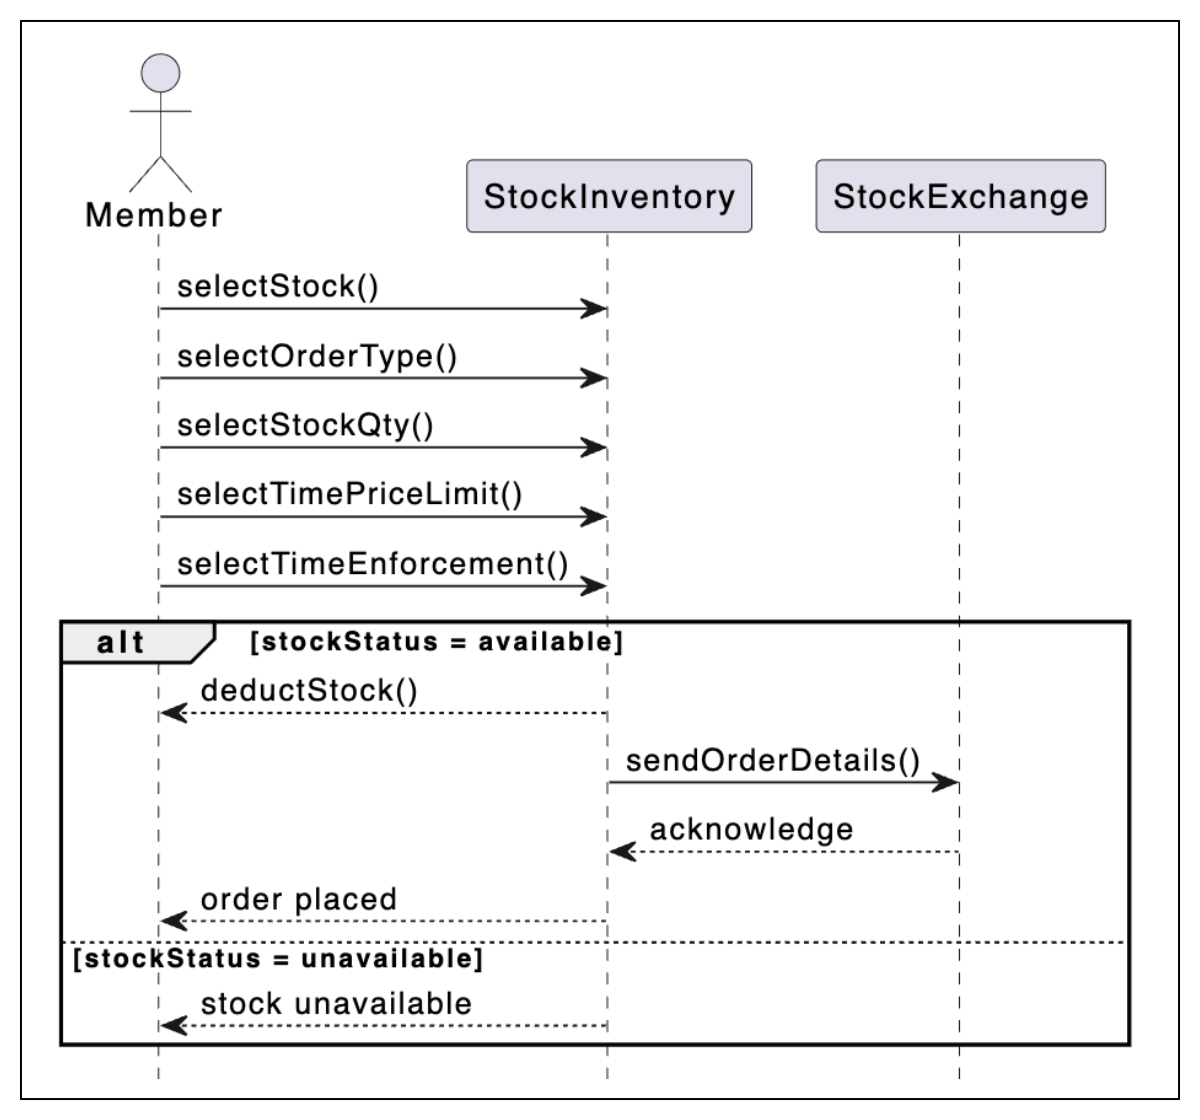
\includegraphics[width=0.5\textwidth]{Images/chapter_23/section_5185398703915008/5438574638792704.png}
 \caption{The sequence diagram for selling a stock}
\end{figure}

Next, let's examine the activity diagrams for an online stock brokerage system to understand its control flow.

% End of section content